\normalsize
\section{Multigrid Method}
The multigrid method has gained popularity since 1980's (See Table \ref{tab:ISI-MG}). It is a fast elliptic equation solver with wide applications in science and engineering areas, including computational fluid dynamics, computational electromagnetics, and structural analysis.
One of the multigrid method implementation for incompressible flow simulations was conducted by Ghia et. al. \cite{Ghia1982}. The advantage of multigrid method over Gauss-Sedel method is analyzed by Demmel \cite{Demmel1997}.
A step-by-step explanation of the multigrid method is provided by Fulton et. al. \cite{Fulton1986}. The standard V-cycle multigrid method as seen in \ref{fig:flowchart-Multigrid} is implemented in this flow model.
\begin{figure}[htbp]
\hspace{0.2in}
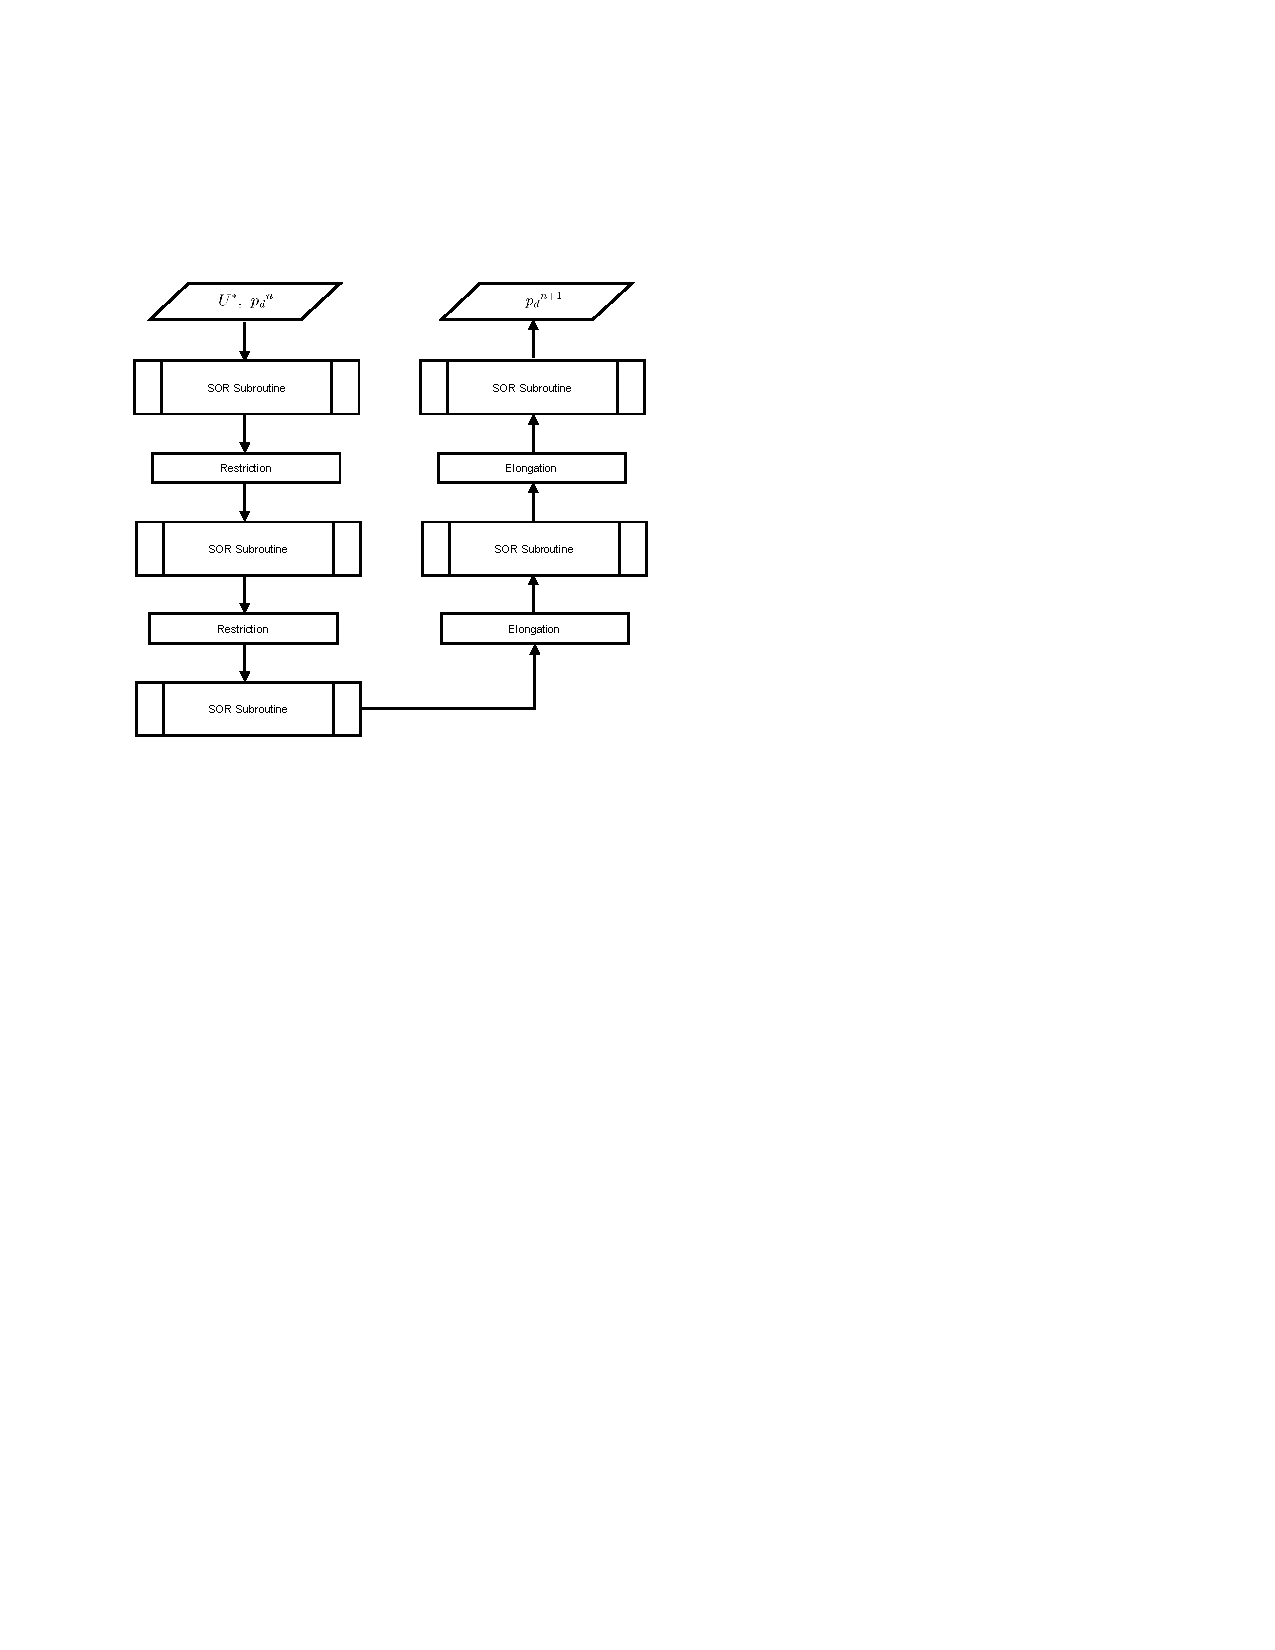
\includegraphics[width=5.2in]{../figures/flowcharts/Multigrid.pdf}
\label{fig:flowchart-Multigrid}
\caption{Flowchart - A three-level V cycle Multigrid method. }
\end{figure}


\begin{table}[hbtp]
\label{tab:ISI-MG}
\begin{center}
\caption{Publications with the keyword "multigrid" on ISI Web of Knowledge, from 2001 to 2005} %(http://www.isiknowledge.com)
\footnotesize
 \begin{tabular}{ccc} \hline %{|c|l|r|r|}
Year    & \# of records  &  Percentage of total 3232 records\\ \hline
1980    &   4   &   0.1238 \%  \\
1981    &   7   &   0.2166 \%  \\
1982    &   33  &   1.0210 \%  \\
1983    &   29  &   0.8973 \%  \\
1984    &   21  &   0.6498 \%  \\
1985    &   31  &   0.9592 \%  \\
1986    &   46  &   1.4233 \%  \\
1987    &   37  &   1.1448 \%  \\
1988    &   53  &   1.6399 \%  \\
1989    &   38  &   1.1757 \%  \\
1990    &   74  &   2.2896 \%  \\
1991    &   131 &   4.0532 \%  \\
1992    &   140 &   4.3317 \%  \\
1993    &   142 &   4.3936 \%  \\
1994    &   130 &   4.0223 \%  \\
1995    &   173 &   5.3527 \%  \\
1996    &   178 &   5.5074 \%  \\
1997    &   178 &   5.5074 \%  \\
1998    &   187 &   5.7859 \%  \\
1999    &   180 &   5.5693 \%  \\
2000    &   196 &   6.0644 \%  \\
2001    &   227 &   7.0235 \%  \\
2002    &   185 &   5.7240 \%  \\
2003    &   217 &   6.7141 \%  \\
2004    &   204 &   6.3119 \%  \\
2005    &   191 &   5.9097 \%  \\
\hline
\end{tabular}
\end{center}
\end{table}
